\documentclass{book}
\usepackage{float}
\usepackage{graphicx}
\title{Figures Mathematical Techniques For Engineers Complex Analysis}
\author{Felix Claeys, Brecht Verbeken, Simon Verbruggen}
\begin{document}
\maketitle
\subsection*{2.1.1 Continuity Definition}
\begin{figure}[H]
\centering
\includegraphics{CH2_Complex_Functions_And_Holomorphy/2.1_Functions_Of_A_Complex_Variable_Limits_And_Continuity/2.1.1_Continuity_Definition/standalone.pdf}
\caption{}
\end{figure}

\section*{2.4 Geometrical Interpretation Of The Complex Derivative}
\begin{figure}[H]
\centering
\includegraphics{CH2_Complex_Functions_And_Holomorphy/2.4_Geometrical_Interpretation_Of_The_Complex_Derivative/standalone.pdf}
\caption{In every point  $g(x_0, y_0)$ of a surface $g(x,y)$, a tangent plane can be drawn (red). The tangent lines $t_x$, $t_y$ are oriented according to the $x$- and $y$-axis, respectively. They have a slope which corresponds to the partial derivatives $\frac{\partial}{\partial x}$ and $\frac{\partial}{\partial y}$, respectively.}
\end{figure}

\section*{3.2 Bilinear transforms}
\begin{figure}[H]
\centering
\includegraphics{CH3_Elementary_Transforms/3.2_Bilinear_transforms/standalone.pdf}
\caption{}
\end{figure}

\subsection*{3.5.1 Exponential function periodicity}
\begin{figure}[H]
\centering
\includegraphics{CH3_Elementary_Transforms/3.5_Exponential_Function/3.5.1_Exponential_function_periodicity/standalone.pdf}
\caption{}
\end{figure}

\subsection*{3.5.2 Exponential function image vertical lines}
\begin{figure}[H]
\centering
\includegraphics{CH3_Elementary_Transforms/3.5_Exponential_Function/3.5.2_Exponential_function_image_vertical_lines/standalone.pdf}
\caption{}
\end{figure}

\subsection*{3.5.3 Exponential function image horizontal lines}
\begin{figure}[H]
\centering
\includegraphics{CH3_Elementary_Transforms/3.5_Exponential_Function/3.5.3_Exponential_function_image_horizontal_lines/standalone.pdf}
\caption{}
\end{figure}

\subsection*{5.1.1}
\begin{figure}[H]
\centering
\includegraphics{CH5_Local_Behaviour_of_Holomorphic_Functions/5.1_Line_integral_of_a_complex_function/5.1.1/standalone.pdf}
\caption{}
\end{figure}

\subsection*{5.2.3}
\begin{figure}[H]
\centering
\includegraphics{CH5_Local_Behaviour_of_Holomorphic_Functions/5.2_Cauchy_Goursat_theorem/5.2.3/standalone.pdf}
\caption{}
\end{figure}

\section*{5.3 Cauchy integral formulas and consequences}
\begin{figure}[H]
\centering
\includegraphics{CH5_Local_Behaviour_of_Holomorphic_Functions/5.3_Cauchy_integral_formulas_and_consequences/standalone.pdf}
\caption{}
\end{figure}

\subsection*{5.4.4}
\begin{figure}[H]
\centering
\includegraphics{CH5_Local_Behaviour_of_Holomorphic_Functions/5.4_Series_of_holomorphic_functions/5.4.4/standalone.pdf}
\caption{}
\end{figure}

\subsection*{5.5.2 Uniqueness of holomorphic functions}
\begin{figure}[H]
\centering
\includegraphics{CH5_Local_Behaviour_of_Holomorphic_Functions/5.5_Zeros_and_poles_of_holomorphic_functions/5.5.2_Uniqueness_of_holomorphic_functions/standalone.pdf}
\caption{}
\end{figure}

\subsection*{5.6.2}
\begin{figure}[H]
\centering
\includegraphics{CH5_Local_Behaviour_of_Holomorphic_Functions/5.6_The_argument_principle/5.6.2/standalone.pdf}
\caption{}
\end{figure}

\subsection*{5.6.3 Argument Principle}
\begin{figure}[H]
\centering
\includegraphics{CH5_Local_Behaviour_of_Holomorphic_Functions/5.6_The_argument_principle/5.6.3_Argument_Principle/standalone.pdf}
\caption{}
\end{figure}

\subsection*{5.6.3 Rouches theorem}
\begin{figure}[H]
\centering
\includegraphics{CH5_Local_Behaviour_of_Holomorphic_Functions/5.6_The_argument_principle/5.6.3_Rouches_theorem/standalone.pdf}
\caption{}
\end{figure}

\end{document}